\section{变量解释、前提和假设}\label{sec:hypothesis}

\subsection{辅助说明}\label{subsec:hypothesis-description}

题干中给出了许多关于路面状况的信息作为辅助说明,我们首先需要对其进行理解。因为世界是三维的,而图片是二维的,故首先需要将给出的三维中的数据信息在二维图像中直观表示,这样便于我们理解。首先我们对路口的平面图进行数据的简单标注,如图\ref{fig:p1}所示。

\begin{figure}[h]
    \centering
    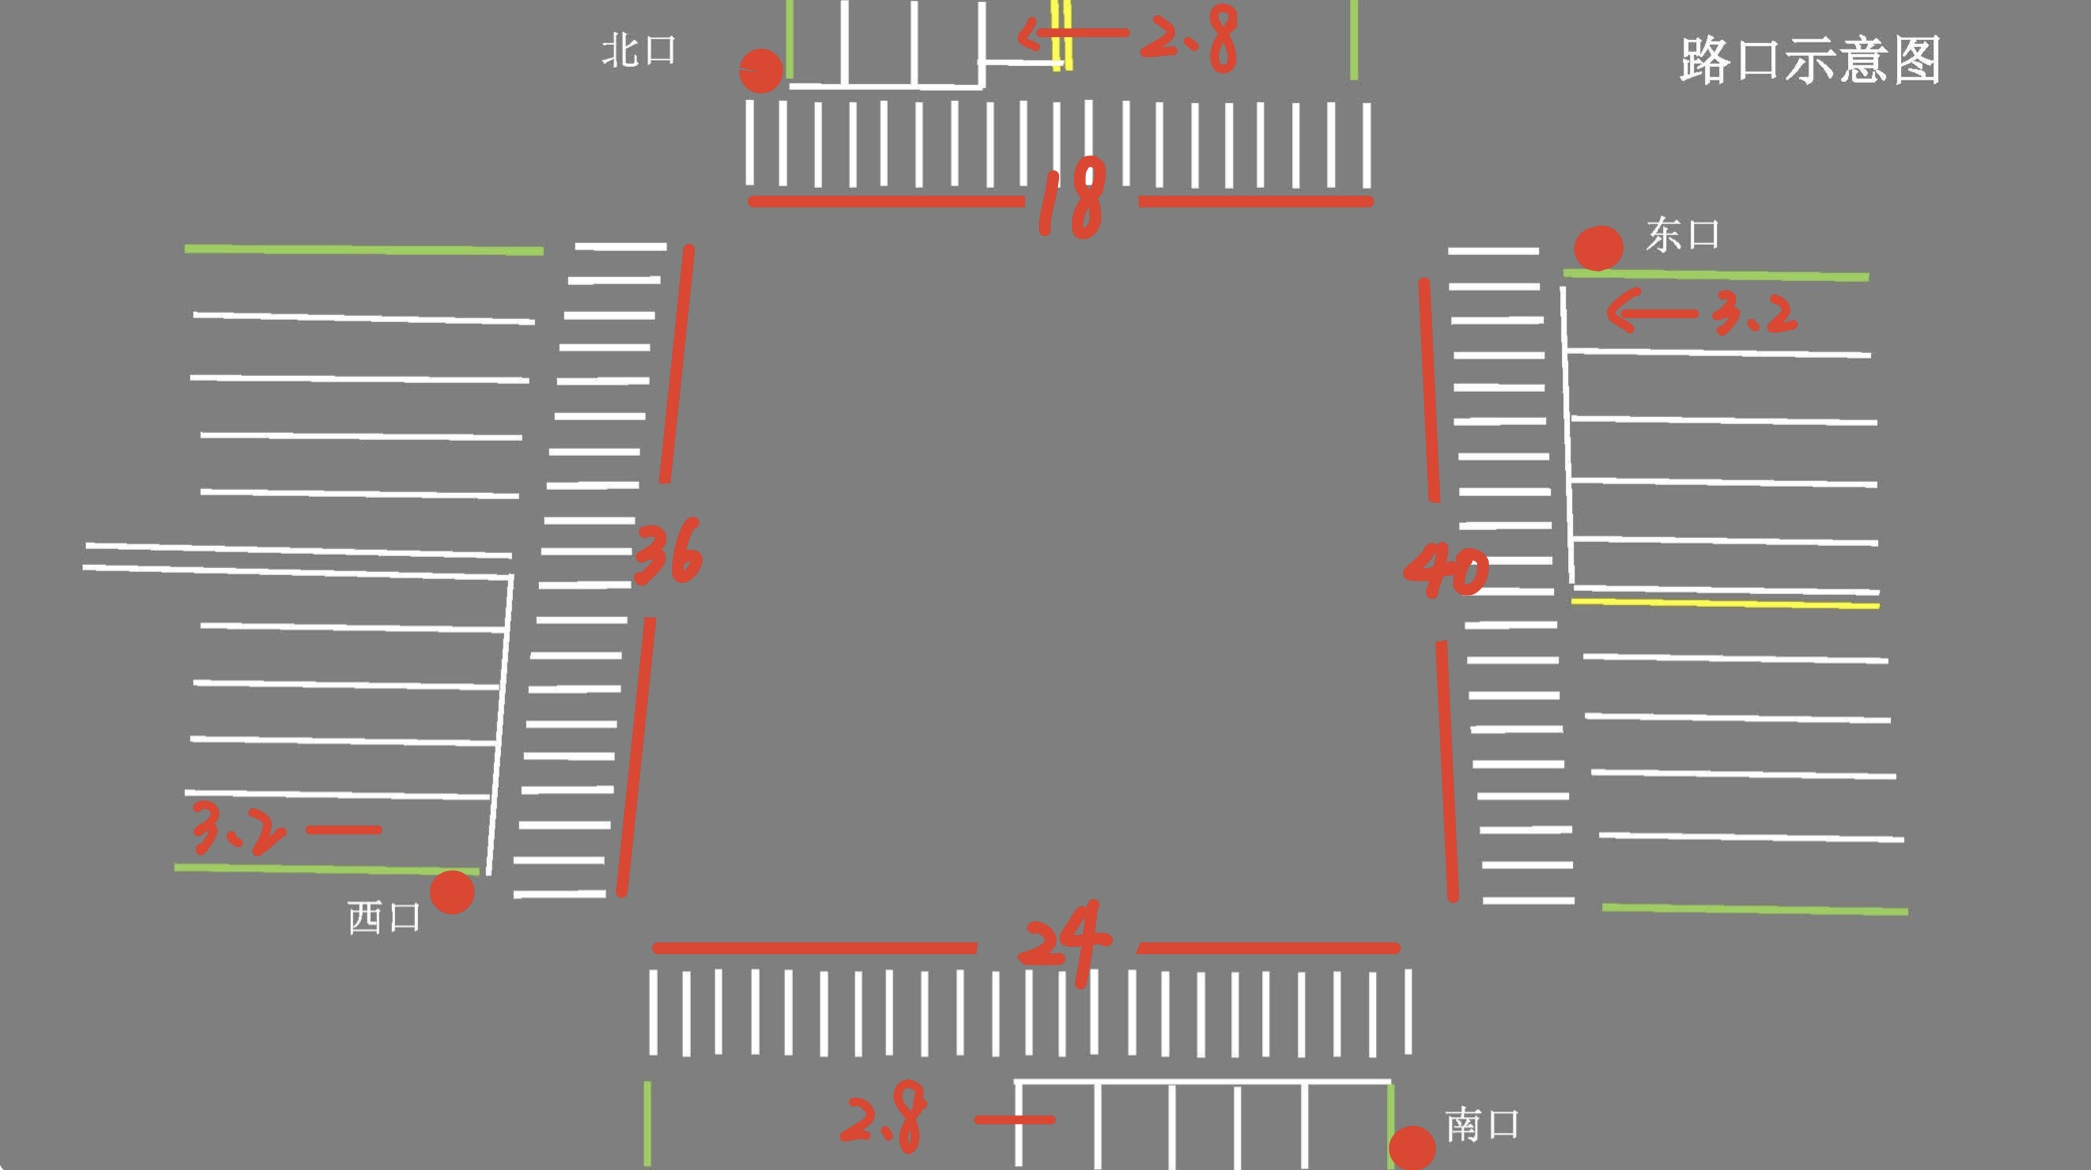
\includegraphics[scale=0.1]{figures/路口阴影图.jpg}
    \caption{路口平面图}
    \label{fig:p1}
\end{figure}

以南口为例,绿线之内为除人行道以外的车道,南口的绿线内总长度为24米,每一个机动车道宽为2.8米。摄像机的位置为图中红点的位置,大致位于路面右侧,交通灯位于对面路的左侧。可以发现,该路口并非一个规则的四边形结构,不仅各边长度不同,各边之间还呈现不同的角度。

考虑到实际生活中的路口形状,不仅有图\ref{fig:p1}所观察出的不规则四边形的特征,还有可能存在诸如在路的拐角出会存在比较大的空白区域这样的问题。考虑了这些因素,我们对图一进行了优化,通过对视频中的路的名称的提取,我们在地图中寻找友谊河路与石杨路交叉路口,通过地图的测距功能得到有关该路口更精确的数据。如下图所示:

\begin{figure}[h]
    \centering
    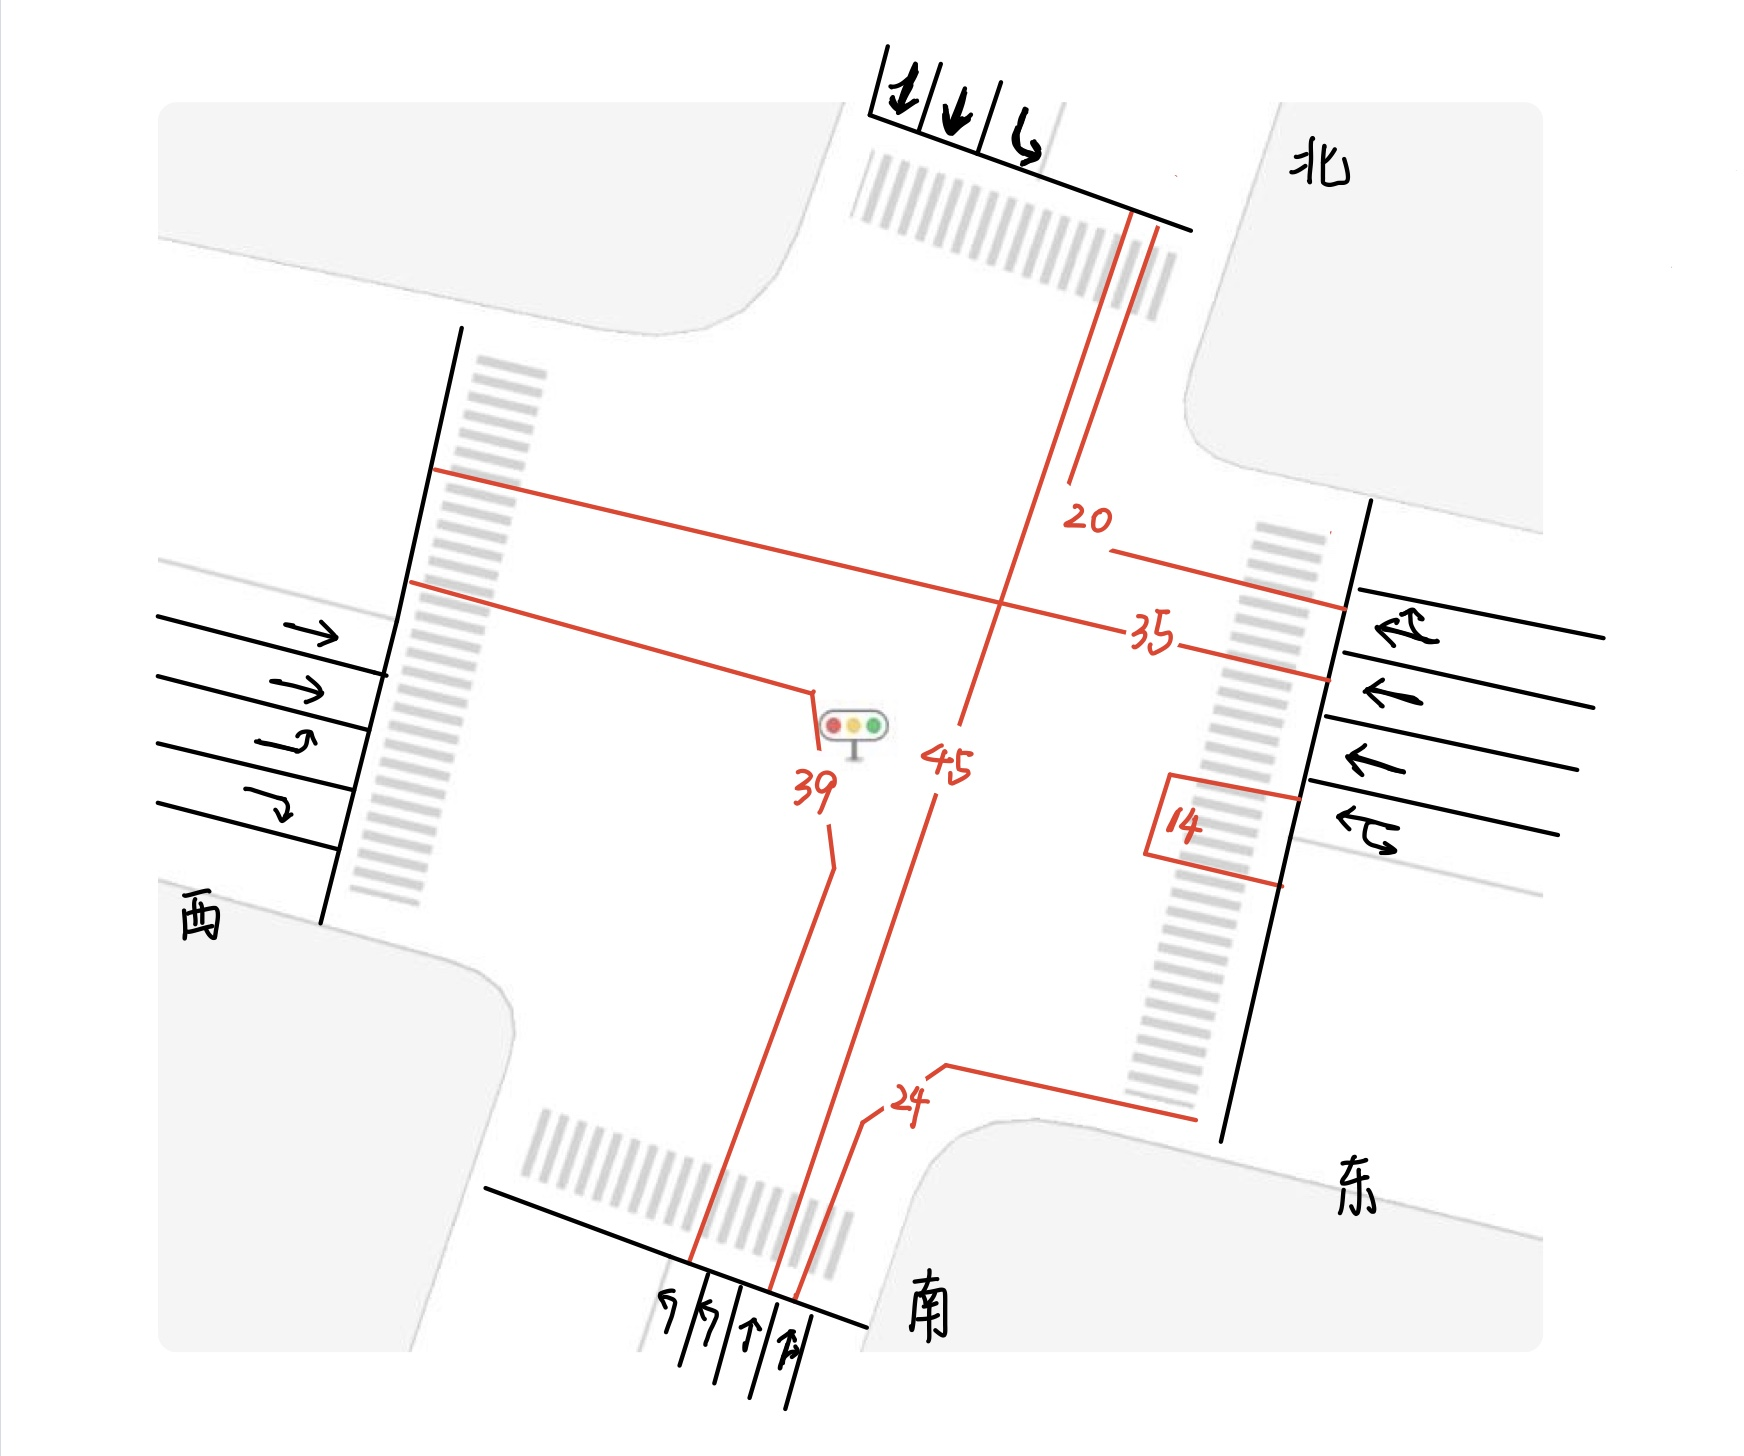
\includegraphics[scale=0.15]{figures/路口平面图.jpg}
    \caption{轨迹距离图}
    \label{fig:p2}
\end{figure}

如\ref{fig:p2}所示,相比上图,显而易见,出现了四个较大面积的拐角,我们将每个路口的行车指示标注其中,粗略测量出了南北方向的停车线之间的长度约为45米,由南口左转至西口停车线的距离约为39米,右转至东口停车线的位置约24米。自东口掉头穿过斑马线的距离约为14米,自东口驶向西口的直线距离约为35米,自东口右转至北口的距离约为20米。收集这部分数据是因为,在车辆位置的判定中,车辆远离停车线30米以上,就视为车辆离开了路口。有了关于路口更精确的数据,可以找到具体处于哪一位置时,视作车辆离开路口。

通过该图,可以简要说明为车道编号的过程中。编号均以最靠中间隔离物的车道为第一车道,以图\ref{fig:p2}的南口为例,最左侧左转车道为南1,第二个左转车道为南2,直行车道为南3,直行加右转车道为南4。

有一些关于摄像机以及路灯高度的数据,我们截取了南口含摄像机的图片,如下所示:

\begin{figure}[h]
    \centering
    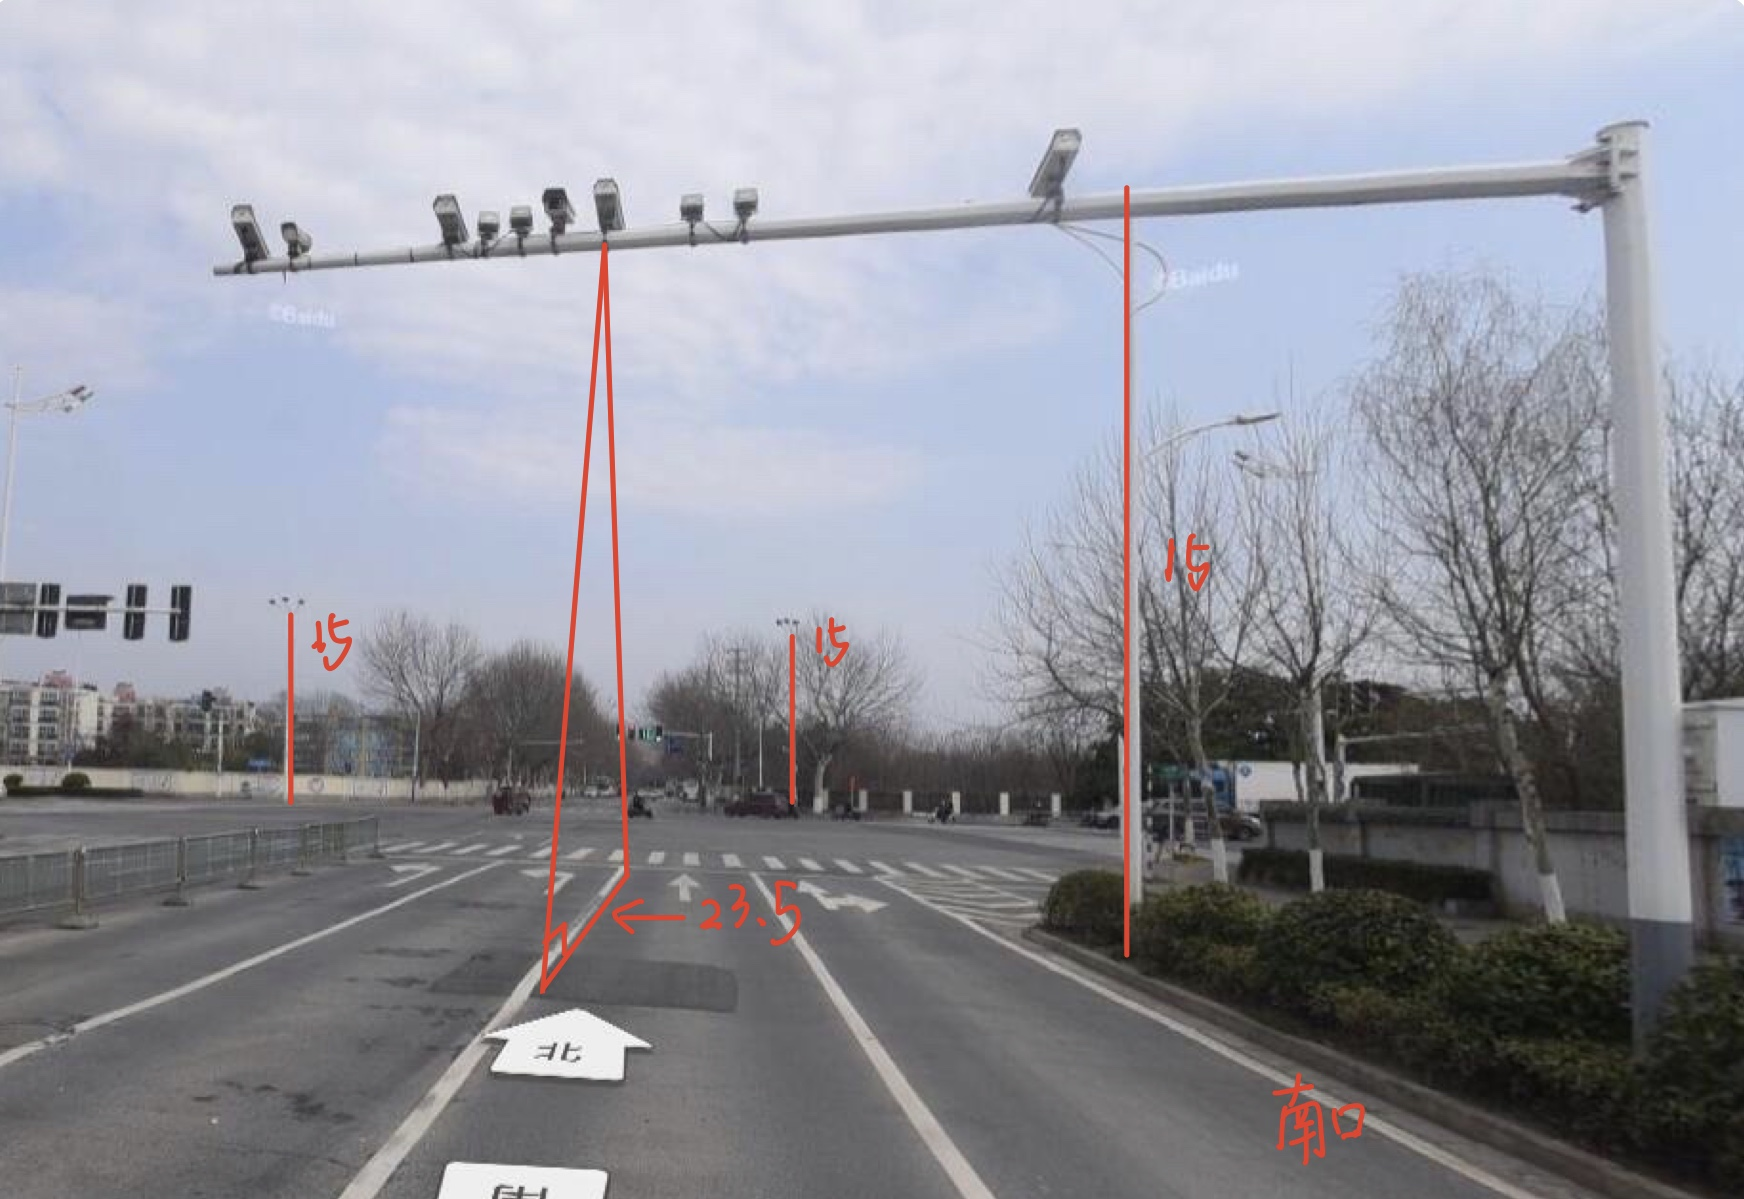
\includegraphics[scale=0.15]{figures/摄像机位置图.jpg}
    \caption{摄像机位置图}
    \label{fig:p3}
\end{figure}

如\ref{fig:p3}所示,这是一张摄于南口的图片,摄像头离地面的高度为6米,自摄像机位置向地面做铅垂线,与地面的交点向停车线作垂线,该垂线即为摄像头的铅直投影点到停车横线的距离,在图中,南口该位置处的距离为23.5米,路口四角处的路灯均为15米高。这些数据,均可用于图片距离向实际距离转化时的参照物。

剩余的辅助说明较好理解,这里作简要介绍。

1.除四角大路灯外,道路上的路灯间距为40米,北口和南口的路灯高10米,东口西口高12米。

2.车辆编号依时间顺序进行,若同时出现,则自画面左侧向右编号,即靠近道路中轴线先编号。

3.车辆位置是指车头距离停车横线的距离,到达停车横线之前为正距离,驶离时为负距离。若车辆驶离停车线30米以上将不再记录距离。

4.车辆的大中小行分类是依据“car”“truck”“bus”标签进行分类的。

\subsection{变量解释}\label{subsec:hypothesis-variables}

通过在视频中的一帧截屏展示的数据,我们对所需要收集的15个变量进行讨论。还有一点要注释的,在附件提供的视频中,视频已经在原基础上5倍速播放。

\begin{figure}[h]
    \centering
    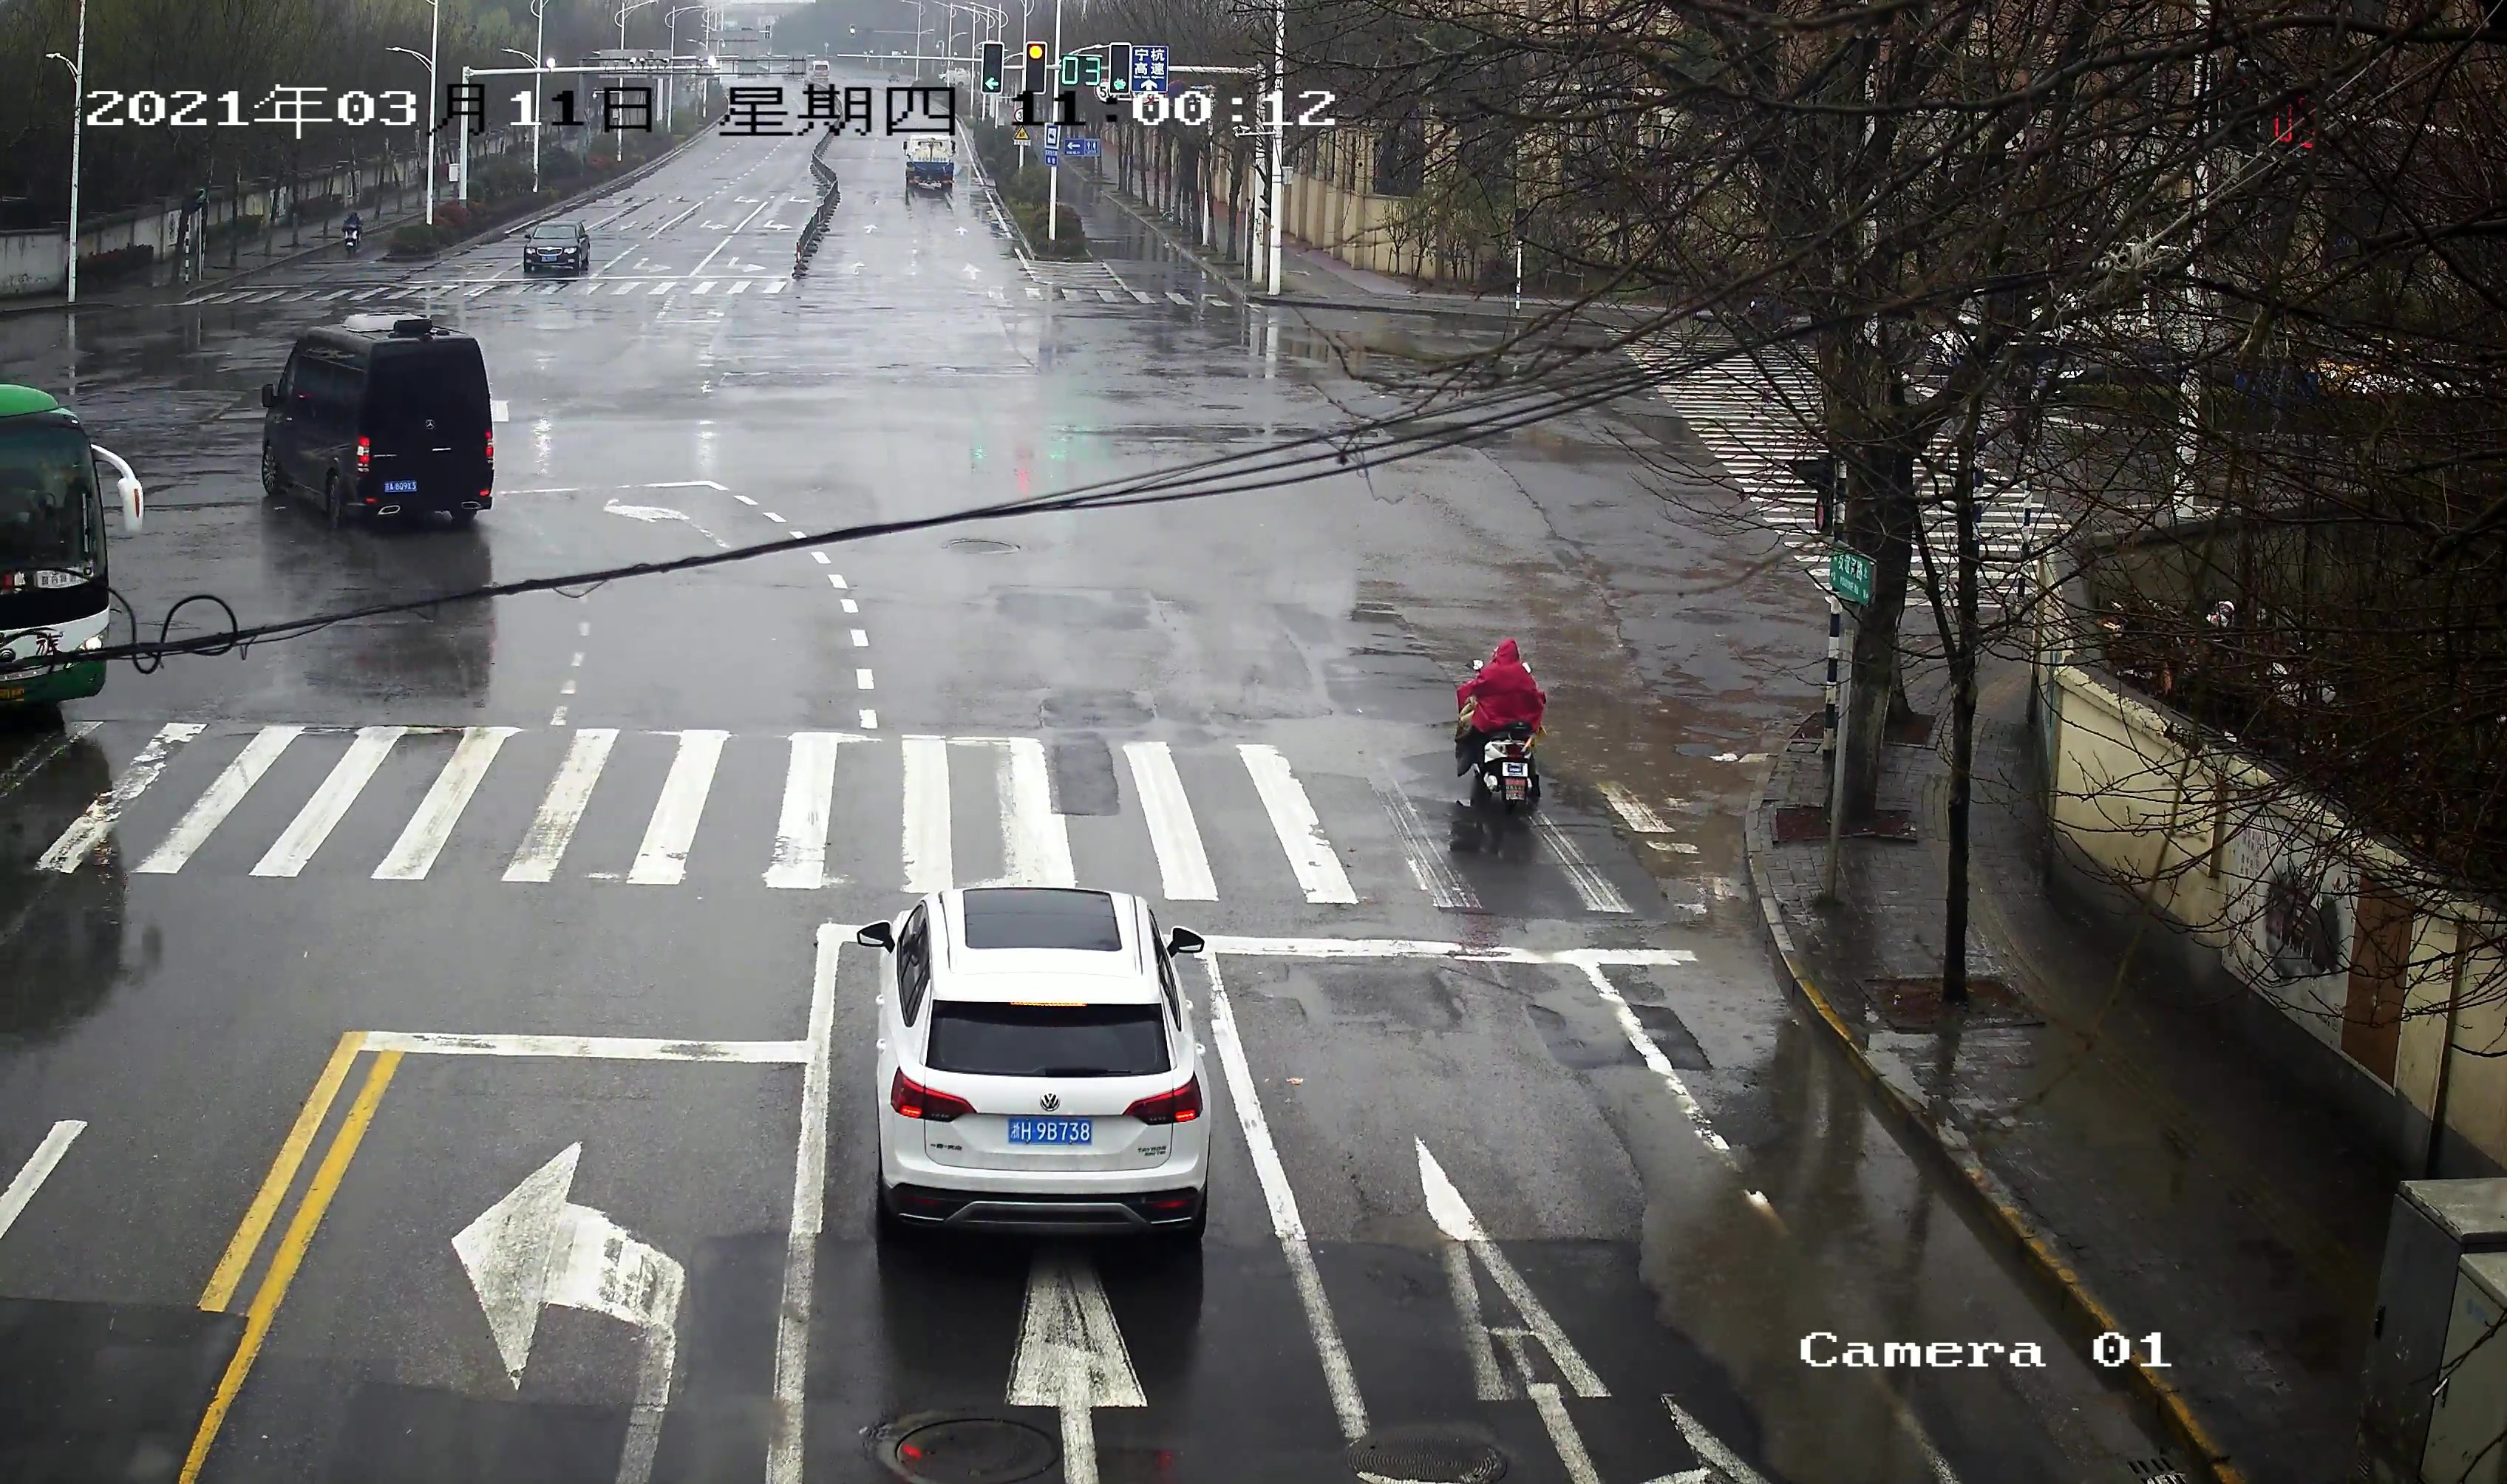
\includegraphics[scale=0.1]{figures/视频截图.jpg}
    \caption{北口视频截图}
    \label{fig:p4}
\end{figure}

如图\ref{fig:p4}所示,左上角有精确的日期和时间的数据,若有车辆从下框进入,即可确定进"进入时刻","进入车道","进入位置",若此时正值红灯,那么车辆在停车线出静止时即可获得"停车时时刻","停车车道","停车时位置","停车时红灯显示时间"等变量,若此时正值绿灯,则这些变量数据为空。

车辆驶离的判定标准为驶离路口30米以上。可以依据前面的手工测量数据,确定驶离位置。以由南向北直行的车辆考虑,行驶至两个停车线距离的$30/45=2/3$时,即可认为是驶离路口。由位置可以确定"驶离路口横线时刻","驶离横线时车道"即为车辆的驶入车道,"驶离横线时绿灯显示时间"和"驶离路口时刻"可由视频时间得出。

进出时间长度由"进入时刻"与“驶离路口横线时刻”作差得出。“进出距离长度”,可由进入位置与驶出位置的轨迹长度确定。

\subsection{前提和假设}\label{subsec:hypothesis-premise}

\begin{figure}[h]
    \centering
    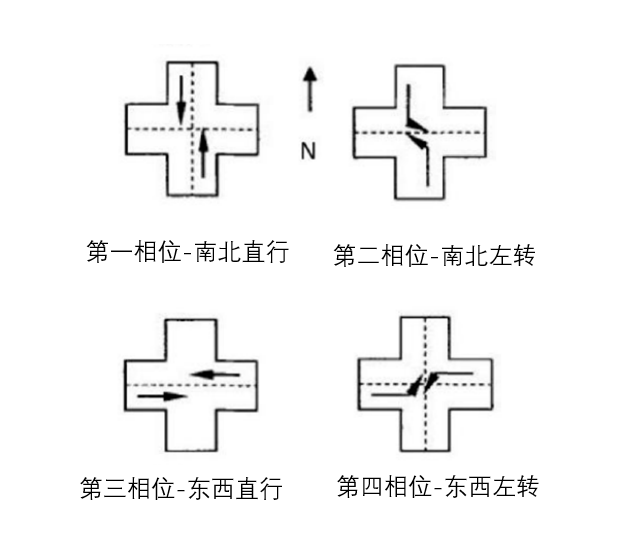
\includegraphics[scale=0.5]{figures/四相相位图.png}
    \caption{相位示意图}
    \label{fig:相位}
\end{figure}

在对于交叉路口的研究中,通常采用四相位控制,本文依照惯例采用如\ref{fig:相位}所示的四相位:东西直行、东西左转、南北直行、南北左转。

在此部分,我们对全文的通用假设进行说明:

(1)任何时候右转的车辆都是可以右转的,对于右转方向的车流,认为其对其他方向的交通流没有影响,在四相位的交通流中,左转方向的交通流,其对整个交通流的影响较大。

(2)在视频中,存在车辆掉头的行为,在本文对于阻碍交通问题的研究中,我们将掉头行为认同为左转,因为和左转需要等待的时间相同,并且驶离路口所用时间和距离接近。

(3)在对路口状况进行抽象建模的过程中,我们可能认为每个周期车辆的到达服从泊松分布。

(4)在本文中识别的路口,由于车辆驶入不含摄像头的一侧,故认为所有识别的车辆不存在数据重合的可能。

(5)本文不考虑行人以及非机动车的影响。
